\section{Franke-function}\label{section:Franke-function}
To develope an understanding of different linear regression methods, the Franke-function will serve as an example. The Franke function is defined as:
\begin{equation}
    \begin{split}
        %\begin{align*}
f(x,y) &= \frac{3}{4}\exp{\left(-\frac{(9x-2)^2}{4} - \frac{(9y-2)^2}{4}\right)}+\frac{3}{4}\exp{\left(-\frac{(9x+1)^2}{49}- \frac{(9y+1)}{10}\right)} \\
&+\frac{1}{2}\exp{\left(-\frac{(9x-7)^2}{4} - \frac{(9y-3)^2}{4}\right)} -\frac{1}{5}\exp{\left(-(9x-4)^2 - (9y-7)^2\right) }.
        %\end{align*}
    \end{split}
\end{equation}
For our purpose we will reduce the function to the interval $x,~y \in [0,~1]$ and add a small stochastic noise $\varepsilon \sim \mathcal{N}(0,~0.1)$ on top. The Frankie is displayed in figure...

% Insert figure


\subsection{Ordinary least squares}
In the first step Ordinary least squares (OLS) will be used to find a function fitting the Franke-function. The mean squared error (MSE) is given by
\begin{equation}
    MSE(\boldsymbol{y},\tilde{\boldsymbol{y}}) = \frac{1}{n}
\sum_{i=0}^{n-1}(y_i-\tilde{y}_i)^2,
\end{equation}
which will be used as a cost function. Different complexity models will be analyzed, calculating the MSE and $R^2$-value depending on the polynomial degree, which are displayed in figure \ref{fig:MSE-R2}. 

% Update figure with other colors, also pdf format
\begin{figure}
    \centering
    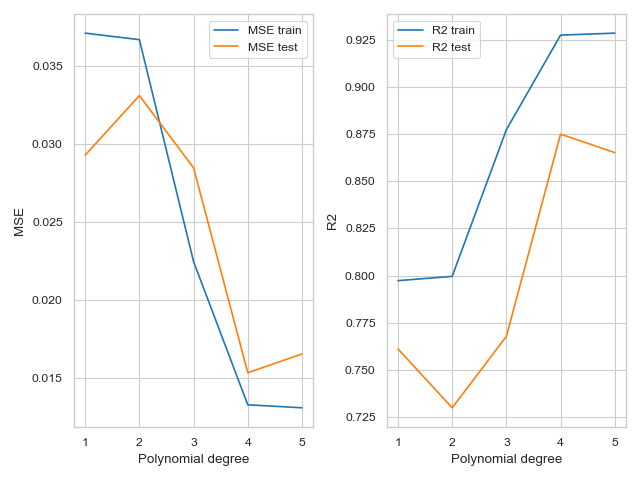
\includegraphics[width=0.9\textwidth]{Figures/1. Franke-function/franke_OLS_mse_r2.png}
    \caption{MSE and $R^2$-value of Ordinary least square fitting the Franke-function for training and test data. }
    \label{fig:MSE-R2}
\end{figure}


The data is split using 70\% as training and 30\% as test data. And the MSE is evaluated for a polynomial polynomial degree up to 5. 





\subsection{Part (d)} \label{section:Exercise 1}
%\setlength{\columnseprule}{1pt}
%\def\columnseprulecolor{\color{Tue-red}} % Creates a red line seperating the colums

%\begin{multicols}{2} % To use a two column page
%\end{multicols}
\begin{equation}
    y = f(x) + \varepsilon, ~~\text{with} ~\varepsilon \sim \mathcal{N}(0, \sigma^2)
\end{equation}
For the Expectation value it is obtained
\begin{equation}
\mathbb{E}[y_i] = \mathbb{E}[f(x) + \varepsilon_i] = 
\underbrace{\mathbb{E}[f(x_i)]}_{\sum_j x_{ij} \beta_j} + 
\underbrace{\mathbb{E}[\varepsilon_i]}_{=0} = 
\sum _j x_{ij}\beta_j = \textbf{X}_{j*} \boldsymbol\beta
\end{equation}
The variance is given by
\begin{equation}
\begin{split}
    \text{Var}(y_i) = \text{Var}[f(x_i) + \varepsilon_i] & = \text{Var}[f(x_i)] +\underbrace{\text{Var}[\varepsilon_i]}_{\sigma^2} + 2\cdot \underbrace{\text{Cov}[f(x_i), \varepsilon_i]}_{=0} \\
   & = \mathbb{E}[f(x_i)^2] - \mathbb{E}[f(x_i)]^2 + \sigma^2 \\
   & = f(x_i)^2 - f(x_i)^2 + \sigma^2 \\
   & = \sigma ^2
    \end{split}
\end{equation}
The expectation value of $\hat\beta$ is given by
\begin{equation}
    \mathbb{E}[\boldsymbol{\hat\beta}] = \mathbb{E}[(\boldsymbol{X}^T\boldsymbol{X})^{-1}\boldsymbol{X}^T\boldsymbol{y}] = (\boldsymbol{X}^T\boldsymbol{X})^{-1} \boldsymbol{X}^T\cdot \underbrace{\mathbb{E}[\boldsymbol{y}]}_{\boldsymbol{X}\boldsymbol\beta} = (\boldsymbol{X}^T\boldsymbol{X})^{-1}\boldsymbol{X}^T\boldsymbol{X}\boldsymbol\beta = \boldsymbol\beta 
\end{equation}
With a variance of 
\begin{equation}
    \begin{split}
    \text{Var}[\boldsymbol{\hat\beta}] = & \mathbb{E}\left\{(\boldsymbol{\hat\beta}-\mathbb{E}[\boldsymbol{\hat\beta}])(\boldsymbol{\hat\beta}-\mathbb{E}[\boldsymbol{\hat\beta}])^T\right\} 
    \\ = & \mathbb{E}\left\{
    \left((\boldsymbol{X}^T\boldsymbol{X})^{-1}\boldsymbol{X}^T\boldsymbol{y} - \boldsymbol\beta\right)
    \left((\boldsymbol{X}^T\boldsymbol{X})^{-1}\boldsymbol{X}^T\boldsymbol{y} - \boldsymbol\beta\right)^T\right\} 
    \\ = & \mathbb{E}\left\{
    (\boldsymbol{X}^T\boldsymbol{X})^{-1}\boldsymbol{X}^T\boldsymbol{y}
    ((\boldsymbol{X}^T\boldsymbol{X})^{-1}\boldsymbol{X}^T\boldsymbol{y})^T
    + \boldsymbol\beta\boldsymbol\beta^T \\
    & - \boldsymbol\beta\boldsymbol{y}^T\boldsymbol{X}(\boldsymbol{X}^T\boldsymbol{X})^{-1}
    -(\boldsymbol{X}^T\boldsymbol{X})^{-1}\boldsymbol{X}^T\boldsymbol{y}\boldsymbol\beta^T\right\}
    \\ = &
    \mathbb{E}\left\{\boldsymbol{X}^T\boldsymbol{X})^{-1} \boldsymbol{X}^T \boldsymbol{y} \boldsymbol{y}^T \boldsymbol{X} (\boldsymbol{X}^T\boldsymbol{X})^{-1} \right\} + \boldsymbol{\beta \beta}^T 
    \\ & - \boldsymbol{\beta}\boldsymbol{\beta}^T \boldsymbol{X}^T\boldsymbol{X} (\boldsymbol{X}^T\boldsymbol{X})^{-1}
    - (\boldsymbol{X}^T\boldsymbol{X})^{-1} \boldsymbol{X}^T\boldsymbol{X}\boldsymbol{\beta}\boldsymbol{\beta}^T\\
    = & \mathbb{E}\left\{\boldsymbol{X}^T\boldsymbol{X})^{-1} \boldsymbol{X}^T \boldsymbol{y} \boldsymbol{y}^T \boldsymbol{X} (\boldsymbol{X}^T\boldsymbol{X})^{-1} \right\}
    - \boldsymbol{\beta \beta}^T \\
    \end{split}
\end{equation}
where 
\begin{equation}
    \mathbb{E}[\boldsymbol{yy}^T] = \boldsymbol{X\beta\beta}^T\boldsymbol{X}
\end{equation}
This yields for the variance
\begin{equation}
    \begin{split}
    \text{Var}[\boldsymbol\hat\beta] = & (\boldsymbol{X}^T\boldsymbol{X})^{-1}(\boldsymbol{X}^T\boldsymbol{X}) \boldsymbol{\beta\beta}^T
    + (\boldsymbol{X}^T\boldsymbol{X})^{-1}\boldsymbol{X}^T\sigma^2\boldsymbol{X} (\boldsymbol{X}^T\boldsymbol{X})^{-1} - \boldsymbol{\beta\beta}^T\\
    = & \sigma^2 (\boldsymbol{X}^T\boldsymbol{X})^{-1}
    \end{split}
\end{equation}

\subsection{Part (e)}

\begin{equation}
    \begin{split}
    \mathbb{E}\left[ (\boldsymbol{y} - \boldsymbol{\tilde{y}})^2\right] = 
    \mathbb{E}\left[ (f(x) + \varepsilon - \boldsymbol{\tilde{y}})^2\right]
    = & \mathbb{E}\left[f(x)^2 + \varepsilon^2 - \boldsymbol{\tilde{y}}^2
    + 2 f(x) \varepsilon - 2f(x) \boldsymbol{\tilde{y}} - 2 \varepsilon \boldsymbol{\tilde{y}}\right]\\
    = & \mathbb{E}\left[ f(x)^2 + \boldsymbol{\tilde{y}}^2  - 2 f(x)\boldsymbol{\tilde{y}}\right] + \sigma^2\\
    \end{split}
\end{equation}
Introducing a 'smart 0', given through the expression $\mathbb{E}[\boldsymbol{\tilde{y}}]- \mathbb{E}[\boldsymbol{\tilde{y}}]= 0$,
we can separate the terms above towards
\begin{equation}
    \begin{split}
        \mathbb{E}\left[ (\boldsymbol{y} - \boldsymbol{\tilde{y}})^2\right] =
        \underbrace{\mathbb{E}[(f(x)-\mathbb{E}[\boldsymbol{\tilde{y}})^2]}_{(\text{Bias}(\boldsymbol{\tilde{y}}))^2}
        + 
        \underbrace{\mathbb{E}[(\boldsymbol{\tilde{y}}}_{\text{Var}(\boldsymbol{\tilde{y}})} - \mathbb{E}[\boldsymbol{\tilde{y}})^2] + 
        \mathbb{E}[(f(x) - \mathbb{E}[\boldsymbol{\tilde{y}}])(\underbrace{\mathbb{E}[\boldsymbol{\tilde{y}}] - \boldsymbol{\tilde{y}})}_{=0}] + \sigma^2
    \end{split}
\end{equation}
Thus we finally obtain
\begin{equation}
    \mathbb{E}\left[ (\boldsymbol{y} - \boldsymbol{\tilde{y}})^2\right] =
    \left[\text{Bias}(\boldsymbol{\tilde{y}})\right]^2 + \text{Var}(\boldsymbol{\tilde{y}}) + \sigma^2
\end{equation}